\section{Durchführung}
\label{sec:Durchführung}

Die Messungen werden mehrfach ausgeführt, um ein Maß für die Zufallsfehler zu bekommen.
Es wird Wechselstrom verwendet. Die Frequenz wird auf $\SI{1}{\kilo\hertz}$ gestellt.
Die Toleranz der Referenzbauteile $R_2$, $C_2$ und $L_2$ liegt bei $\pm \SI{0.2}{\percent}$, wobei diese in der Auswertung vernachlässigt wird, da der Fehler der Ergebnisse über die Standardabweichung der Mittelwerte gebildet wird.

\subsection{Bestimmung von Widerständen mittels Wheatstone-Brücke}
Mit der Wheatoneschen Brückenschaltung (s. Abb. \ref{wheatstone}) werden im ersten Aufgabenteil zwei unbekannte Widerstände ausgemessen.
Das Potentiometer hat einen Gesamtwiderstand von $\SI{1}{\kilo\ohm}$.
Der Drehknopf des Potentiometers wird für jeden der beiden Widerstände 
jeweils so eingestellt, dass die Brückenspannung Null wird. 
Der am Drehknopf angezeigte Wert ist der Wert für $R_3$ in Promille. 
$R_4$ ergibt sich, indem $R_3$ von $\num{1000}$ abgezogen wird.
Der Widerstand $R_2$ wird hier mehrfach variiert. Für jeden unbekannten Widerstand $R_X$
werden drei unterschiedliche Widerstände $R_2$ benutzt.
\begin{figure}
    \centering
    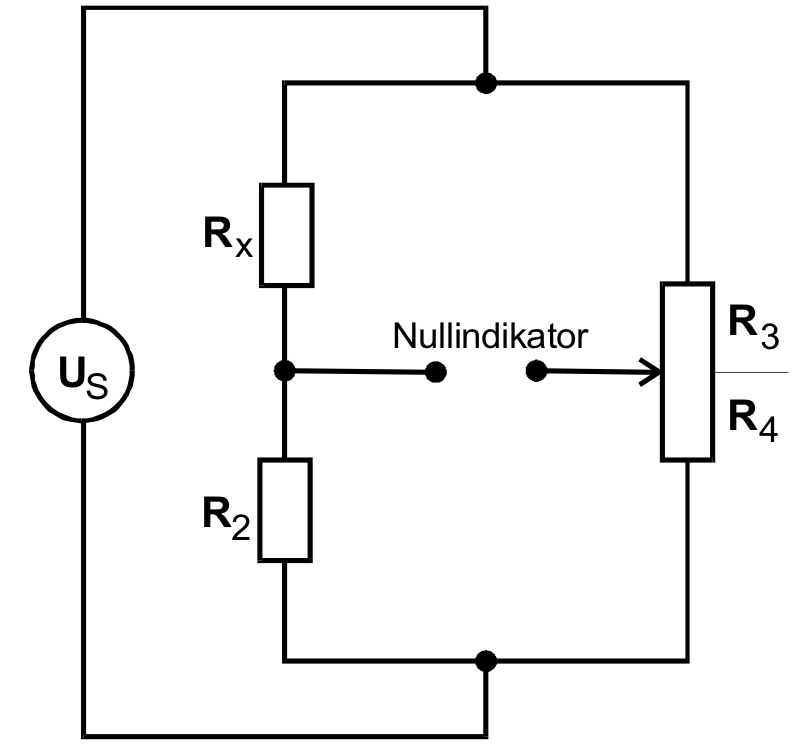
\includegraphics[width=5cm, height=5cm]{build/wheatstone.png}
    \caption{Wheatstonesche Brücke. Diese Schaltung wird zur Bestimmung
    des Widerstandes $R_X$ genutzt. Die Widerstände $R_3$ und $R_4$
    sind als Potentiometer ausgebildet. $R_2$ ist bekannt.}%ausgebildet?
    \label{wheatstone}
\end{figure}

\subsection{Bestimmung von Kapazitäten mittels Kapazitätsmessbrücke}
Als nächstes sollen anhand einer Kapazitätsmessbrücke die Kapazität und der 
Verlustwiderstand von einem Kondensator gemessen werden.
\newline
Zunächst wird das Minimum der Brückenspannung mittels $R_3/R_4$ eingestellt.
Anschließend wird $R_2$ so justiert, dass die Spannung kleiner wird.
Die Stellglieder werden weiterhin alternierend so justiert, dass die
Brückenspannung Null wird. Die Werte für $R_2$ und $R_3$ können an den
Potentiometern abgelesen werden. $R_4$ ergibt sich, indem $R_3$ von 
$\num{1000}$ abgezogen wird.
\begin{figure}
    \centering
    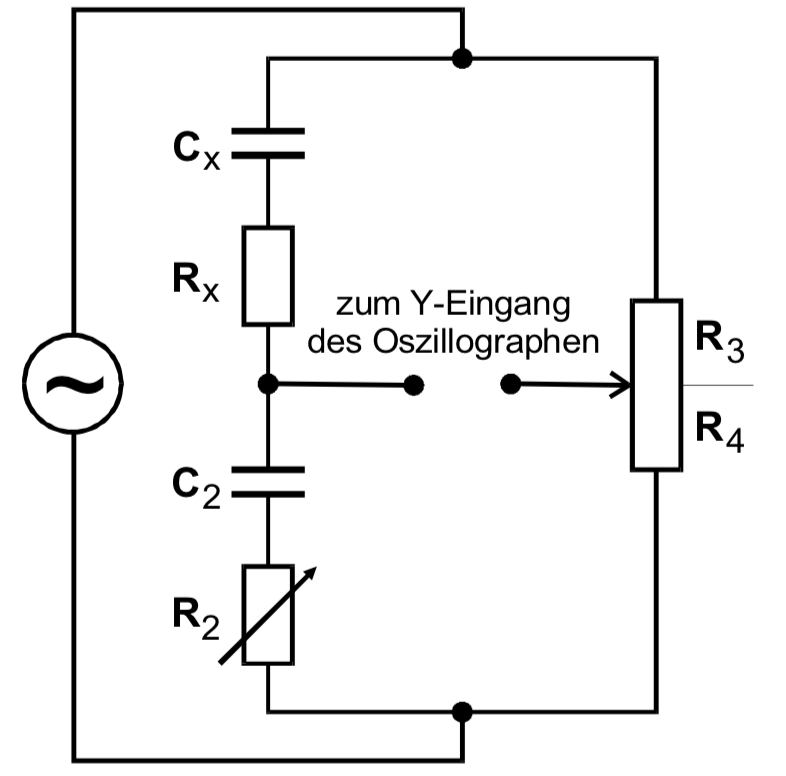
\includegraphics[width=5cm, height=5cm]{build/kapazitaet.png}
    \caption{Kapazitätsmessbrücke. Diese Schaltung wird zur Bestimmung
    der Kapazität $C_X$ genutzt. Der Widerstand $R_X$ folgt aus dem
    Ersatzschaltbild des Kondensators. Die Widerstände $R_3$ und $R_4$
    sind als Potentiometer ausgebildet. Der Widerstand $R_2$ ist
    verstellbar. $C_2$ ist bekannt.}
    \label{kapazitaet}
\end{figure}

\subsection{Bestimmung von Induktivitäten mittels Induktivitätsmessbrücke}
Die Induktivität und der Verlustwiderstand einer unbekannten Spule werden 
an einer Induktivitätsmessbrücke gemessen.
\newline
Zunächst wird das Minimum der Brückenspannung mittels $R_3/R_4$ eingestellt.
Anschließend wird $R_2$ so justiert, dass die Spannung kleiner wird.
Die Stellglieder werden weiterhin alternierend so justiert, dass die
Brückenspannung Null wird. Die Werte für $R_2$ und $R_3$ können an den
Potentiometern abgelesen werden. $R_4$ ergibt sich, indem $R_3$ von 
$\num{1000}$ abgezogen wird.
\begin{figure}
    \centering
    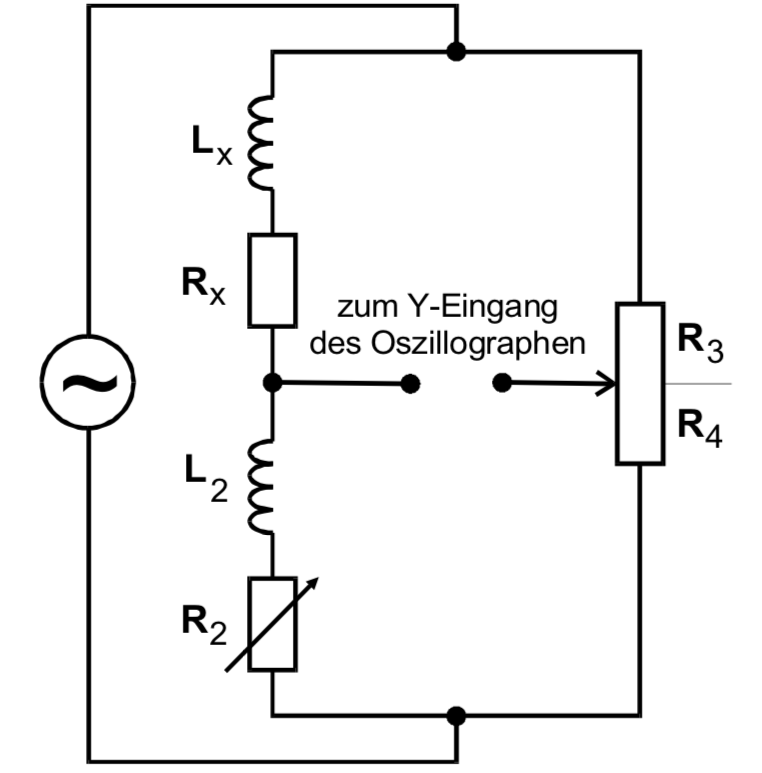
\includegraphics[width=5cm, height=5cm]{build/induktivitaet.png}
    \caption{Induktivitätsmessbrücke. Diese Schaltung wird zur Bestimmung
    von $L_X$ genutzt. Der Widerstand $R_X$ folgt aus dem
    Ersatzschaltbild der Induktivität (Spule). Die Widerstände $R_3$ und $R_4$
    sind als Potentiometer ausgebildet. Der Widerstand $R_2$ ist
    verstellbar. $L_2$ ist bekannt.}
    \label{induktivitaet}
\end{figure}

\subsection{Bestimmung von Induktivitäten mittels Maxwell-Brücke}
Anschließend wird die Spule ein zweites Mal mit Hilfe der Maxwell-Brücke durchgemessen.
\newline
$R_3$ und $R_4$ werden alternierend so eingestellt, dass die Brückenspannung
Null wird. 
\begin{figure}
    \centering
    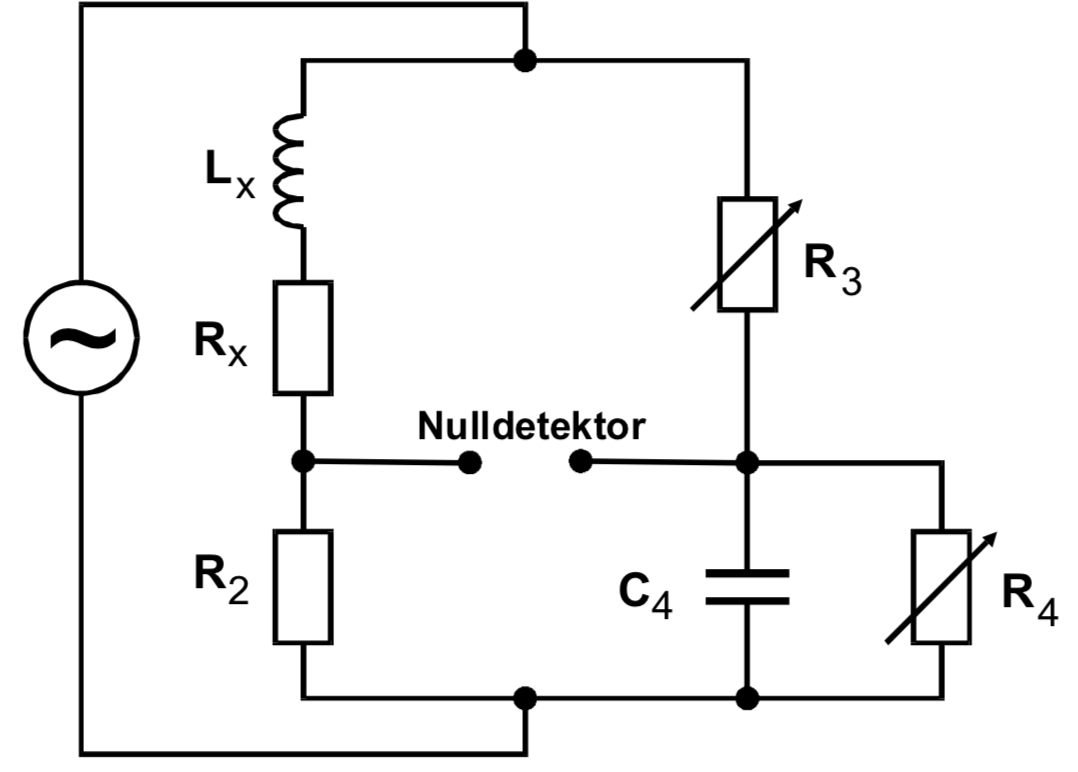
\includegraphics[width=5cm, height=5cm]{build/maxwell.png}
    \caption{Maxwell-Brücke. Diese Schaltung wird zur Bestimmung
    von $L_X$ genutzt. Der Widerstand $R_X$ folgt aus dem
    Ersatzschaltbild der Induktivität (Spule). Die Widerstände
    $R_3$ und $R_4$ sind verstellbar. $R_2$ und $C_4$ sind bekannt.}
    \label{maxwell}
\end{figure}

\subsection{Bestimmung der Frequenzabhängigkeit der Brückenspannung mittels Wien-Robinson-Brücke}
%Die Frequenzabhängigkeit der Brückenspannung in einer Wien-Robinson-Brücke wird mit dem Theoriewert verglichen. 
Um die Frequenzabhängigkeit der Brückenspannung $U_{Br}$ zu messen, wird eine 
Wien-Robinson-Brücke verwendet.
\newline
Die eingestellten Frequenzen liegen in einem Bereich von $\num{20}$ bis $\SI{30000}{\hertz}$.
Die Werte für die Brückenspannung bei bestimmten eingestellten Frequenzen
lassen sich am Oszillographen ablesen. %Oszillograph?
Die eingestellte Spannung $U_S$ lässt sich ebenfalls mit dem Oszillographen
bestimmen.
\begin{figure}
    \centering
    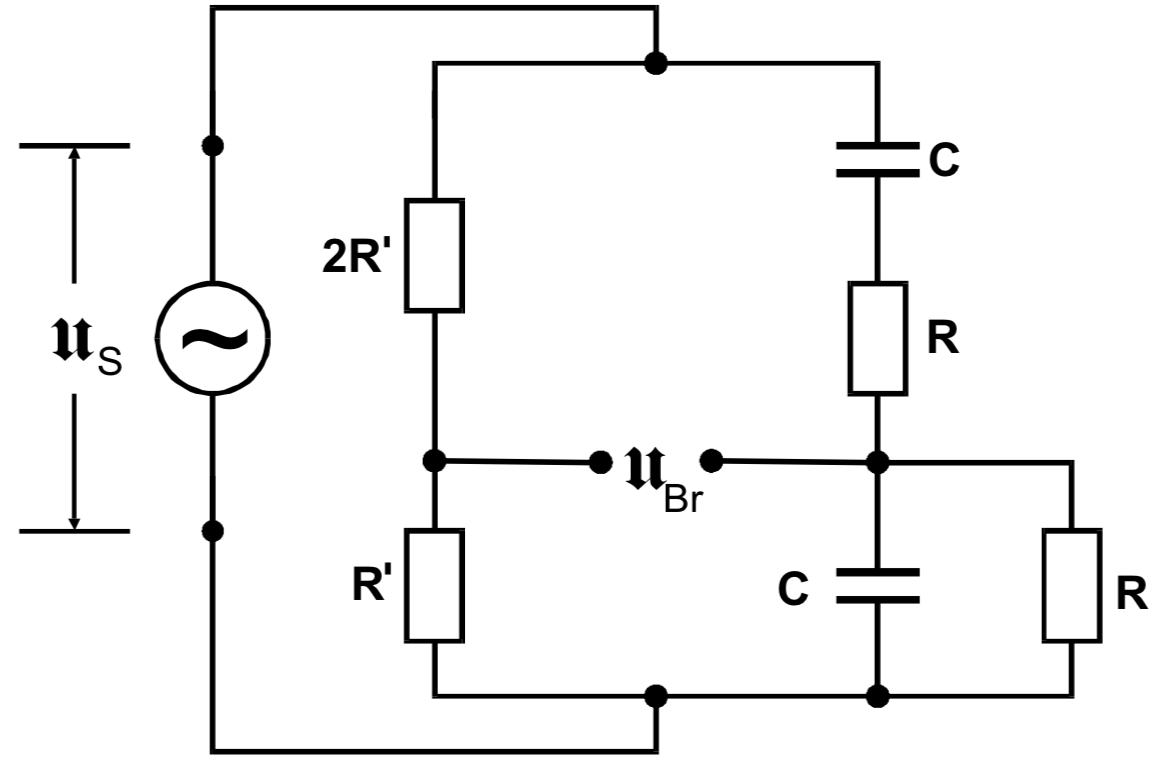
\includegraphics[width=5cm, height=5cm]{build/wien-robinson.png}
    \caption{Wien-Robinson-Brücke. Diese Schaltung wird zur Bestimmung
    der Brückenspannung $U_B$ genutzt. Die Widerstände $R'$ und $R$,
    sowie die Kapazität $C$ sind bekannt.}
    \label{wien-robinson}
\end{figure}

\subsection{Bestimmung des Klirrfaktors}
Als letztes soll der Klirrfaktor des verwendeten Generators bestimmt werden.
\newline
Dabei wird das Minimum der Brückenspannung $U_{Br}$ bestimmt.
Daraus lässt sich der Klirrfaktor errechnen.
%und der Quotient aus der vorhandenen Oberwellen und der Grundwelle bestimmt.

